\documentclass[aspectratio=169,11pt]{beamer}

\def\courseTitle{Industrial Security (Bachelor)}
\def\courseSubtitle{Section 09 -- Standards, Compliance, Governance}
\def\sectionNumber{09}
\def\sectionTitle{Standards, Compliance, and Governance}

% =====================================================================
% Industrial Security lecture series -- modern Beamer preamble.
%
% Each slide deck must define the following BEFORE \input{}-ing this:
%   \def\courseTitle{...}        e.g. Industrial Security (Bachelor)
%   \def\courseSubtitle{...}     e.g. Section 3 -- Network Architecture
%   \def\sectionNumber{...}      e.g. 03
%   \def\sectionTitle{...}       e.g. Industrial Network Architectures
%
% Optional:
%   \def\courseAuthor{...}       defaults to "Lecture Notes"
%   \def\courseInstitute{...}    defaults to "Department of Computer Science"
%   \def\companyLogo{...}        path to a logo image (PDF/PNG/JPG).
%
% Callout macros (use anywhere inside a frame):
%   \begin{notebox}{title}      ... \end{notebox}
%   \begin{importantbox}{title} ... \end{importantbox}
%   \begin{warningbox}{title}   ... \end{warningbox}
%   \begin{tipbox}{title}       ... \end{tipbox}
%   \begin{defbox}{title}       ... \end{defbox}
%   \begin{takeawaybox}{title}  ... \end{takeawaybox}
%   \begin{quotebox}            ... \end{quotebox}
% =====================================================================

% --- Speaker-notes mode (toggled by Makefile via -usepretex) ----------
% When notesmode=1, build a side-by-side slide+notes PDF for the
% lecturer. When unset/0, build the clean slides-only PDF.
\providecommand{\notesmode}{0}
\ifnum\notesmode=1
  \usepackage{pgfpages}
  \setbeameroption{show notes on second screen=right}
  \setbeamerfont{note page}{size=\small}
\fi

\usepackage[utf8]{inputenc}
\usepackage[T1]{fontenc}
\usepackage[english]{babel}
% Modern type pair: IBM Plex Sans for text, IBM Plex Mono for code.
% Math stays in lmodern; Plex is the dominant family on every text frame.
\usepackage{plex-sans}
\usepackage{plex-mono}
\renewcommand{\familydefault}{\sfdefault}
\usepackage[activate={true,nocompatibility},final,tracking=true,kerning=true,spacing=true,factor=1100,stretch=10,shrink=10]{microtype}
\usepackage{graphicx}
\usepackage{listings}
\usepackage{xcolor}
\usepackage{colortbl}
\usepackage{tikz}
\usepackage{booktabs}
\usepackage{array}
\usepackage{hyperref}
\usepackage{amsmath}
\usepackage{amssymb}
\usepackage{tcolorbox}
\tcbuselibrary{skins, breakable, raster}
\usepackage{fontawesome5}

% =====================================================================
% Shared TikZ styles for the Industrial Security lecture series.
% Loaded by every slide deck and exercise sheet that uses TikZ.
% =====================================================================

\usetikzlibrary{
  arrows.meta,
  shapes,
  shapes.geometric,
  shapes.symbols,
  shapes.multipart,
  positioning,
  fit,
  calc,
  backgrounds,
  decorations.pathmorphing,
  decorations.pathreplacing,
  decorations.text,
  patterns,
  matrix,
  shadows
}

% --- colour palette --------------------------------------------------
\definecolor{isOT}{HTML}{1F4E79}     % OT (deep blue)
\definecolor{isIT}{HTML}{6F2DA8}     % IT (purple)
\definecolor{isSafety}{HTML}{C00000} % safety red
\definecolor{isNet}{HTML}{2E7D32}    % network green
\definecolor{isAttack}{HTML}{B23A48} % attack red
\definecolor{isAccent}{HTML}{E08E0B} % amber
\definecolor{isMute}{HTML}{6B6B6B}   % grey
\definecolor{isLight}{HTML}{EDF2F8}  % light background
\definecolor{isPLC}{HTML}{2C5282}
\definecolor{isHMI}{HTML}{2F855A}
\definecolor{isSCADA}{HTML}{6B46C1}

% --- generic node styles --------------------------------------------
\tikzset{
  isnode/.style={
    draw, rounded corners=2pt, minimum height=8mm, minimum width=18mm,
    font=\small, align=center, thick
  },
  isbox/.style={isnode, fill=isLight},
  plc/.style={isnode, fill=isPLC!15, draw=isPLC, thick},
  hmi/.style={isnode, fill=isHMI!15, draw=isHMI, thick},
  scada/.style={isnode, fill=isSCADA!15, draw=isSCADA, thick},
  sensor/.style={isnode, fill=isNet!10, draw=isNet, minimum height=6mm, minimum width=14mm, font=\scriptsize},
  actuator/.style={isnode, fill=isAccent!15, draw=isAccent, minimum height=6mm, minimum width=14mm, font=\scriptsize},
  firewall/.style={isnode, fill=isAttack!15, draw=isAttack, thick},
  server/.style={isnode, fill=isMute!15, draw=isMute!80, thick},
  switch/.style={isnode, fill=isLight, draw=black!60, minimum height=6mm, minimum width=14mm, font=\scriptsize},
  workstation/.style={isnode, fill=white, draw=isOT, thick},
  attacker/.style={isnode, fill=isAttack!20, draw=isAttack, thick, font=\small\bfseries},
  inetnode/.style={draw, ellipse, minimum width=24mm, minimum height=10mm, font=\scriptsize, fill=isLight, thick},
  process/.style={isnode, fill=isOT!15, draw=isOT, thick, minimum width=24mm},
  zone/.style={
    draw, rounded corners=4pt, thick, dashed, inner sep=4mm
  },
  conduit/.style={-{Stealth[length=2.5mm]}, thick, isNet!80!black},
  attack/.style={-{Stealth[length=2.5mm]}, thick, isAttack, dashed},
  flow/.style={-{Stealth[length=2.5mm]}, thick, isOT!70!black},
  netline/.style={thick, black!60},
  axisline/.style={-{Stealth[length=2mm]}, thick, black!70},
  tag/.style={font=\scriptsize\itshape, fill=white, inner sep=1pt},
  level/.style={
    draw, fill=isLight, minimum width=0.85\linewidth, minimum height=8mm,
    font=\small, anchor=west
  },
  brace/.style={decorate, decoration={brace, amplitude=4pt, raise=2pt}},
  legendbox/.style={draw, rounded corners=2pt, fill=isLight, inner sep=2mm, font=\scriptsize, align=left}
}

% --- handy macros ----------------------------------------------------
% \plcicon, \hmiicon etc as simple labelled boxes; useful inline.
\newcommand{\plcicon}[1][PLC]{\tikz[baseline=-0.6ex]{\node[plc, minimum width=10mm, minimum height=5mm, font=\scriptsize, inner sep=1pt]{#1};}}
\newcommand{\hmiicon}[1][HMI]{\tikz[baseline=-0.6ex]{\node[hmi, minimum width=10mm, minimum height=5mm, font=\scriptsize, inner sep=1pt]{#1};}}
\newcommand{\fwicon}[1][FW]{\tikz[baseline=-0.6ex]{\node[firewall, minimum width=10mm, minimum height=5mm, font=\scriptsize, inner sep=1pt]{#1};}}


\graphicspath{{.}{../../../template/}}

% --- defaults --------------------------------------------------------
\providecommand{\courseAuthor}{Lecture Notes}
\providecommand{\courseInstitute}{Department of Computer Science}
\providecommand{\companyLogo}{logo}

% --- modern palette --------------------------------------------------
\definecolor{slideAccent}{HTML}{1F4E79}       % primary navy
\definecolor{slideSecondary}{HTML}{E08E0B}    % amber accent

% --- Corporate branding overrides ------------------------------------
% A user-editable `branding.tex` at the repo root can override the
% logo path, author/institute lines, and brand colours. If the file is
% missing the built-in defaults above stay in effect.
\IfFileExists{../../../branding.tex}{% =====================================================================
% Corporate / institutional branding -- single file to customise the
% look of the entire course (slides, notes, exercises, labs).
%
% HOW TO REBRAND IN UNDER A MINUTE:
%   1. Replace `branding/logo.pdf` with your own logo
%      (PDF preferred; PNG and JPG also work -- name it `logo.<ext>`).
%   2. (Optional) change the two colours below to your brand palette.
%   3. (Optional) override the author/institute lines below.
%   4. Re-run `make` at the repo root. That's it.
%
% Everything in this file has sensible defaults; you can delete a line
% to fall back to the built-in defaults, or comment it out.
%
% This file is loaded automatically by the slides, exercise, and lab
% preambles -- you never need to \input it manually.
% =====================================================================

% --- Logo --------------------------------------------------------------
% Path is resolved from each leaf-build directory; the default points at
% the shared `branding/` folder at the repo root. If you put your logo
% somewhere else, set the full or relative path here (without extension):
\renewcommand{\companyLogo}{../../../branding/logo}

% --- Author / institute (appears on the title page footer) ------------
\renewcommand{\courseAuthor}{}
\renewcommand{\courseInstitute}{}

% --- Brand colours ----------------------------------------------------
% slideAccent      = primary brand colour (title bands, accent rule)
% slideSecondary   = secondary brand colour (section badge, highlight)
% Both use HTML hex codes. Keep enough contrast against white text.
\definecolor{slideAccent}{HTML}{00205B}      % deep navy
\definecolor{slideSecondary}{HTML}{00A0DC}   % light blue accent
}{}
\definecolor{slideTitle}{HTML}{0F2A44}        % near-black navy
\definecolor{slideMuted}{HTML}{6B6B6B}
\definecolor{slideBg}{HTML}{FFFFFF}
\definecolor{slidePanel}{HTML}{F4F7FB}
\definecolor{slideRule}{HTML}{D6DEE8}

% Callout colours
\definecolor{calNote}{HTML}{1F4E79}
\definecolor{calImportant}{HTML}{B23A48}
\definecolor{calWarning}{HTML}{C77700}
\definecolor{calTip}{HTML}{2E7D32}
\definecolor{calDef}{HTML}{6B46C1}
\definecolor{calTake}{HTML}{0F2A44}

% --- beamer theme ---------------------------------------------------
\useinnertheme{rectangles}
\usefonttheme{professionalfonts}

\setbeamertemplate{navigation symbols}{}
\setbeamertemplate{itemize items}[circle]
\setbeamertemplate{enumerate items}[default]
\setbeamertemplate{section in toc}[ball numbered]
\setbeamercolor{section in toc}{fg=slideTitle}

% Colours
\setbeamercolor{normal text}{fg=slideTitle, bg=slideBg}
\setbeamercolor{title}{fg=slideAccent}
\setbeamercolor{subtitle}{fg=slideMuted}
\setbeamercolor{frametitle}{fg=slideAccent}
\setbeamercolor{structure}{fg=slideAccent}
\setbeamercolor{itemize item}{fg=slideAccent}
\setbeamercolor{itemize subitem}{fg=slideSecondary}
\setbeamercolor{block title}{fg=white, bg=slideAccent}
\setbeamercolor{block body}{fg=slideTitle, bg=slidePanel}
\setbeamercolor{alerted text}{fg=slideSecondary}

% Fonts
\setbeamerfont{title}{series=\bfseries, size=\Large}
\setbeamerfont{subtitle}{series=\mdseries, size=\normalsize}
\setbeamerfont{frametitle}{series=\bfseries, size=\large}
\setbeamerfont{block title}{series=\bfseries, size=\normalsize}
\setbeamerfont{footline}{size=\tiny}

% --- frametitle: title bar + accent underline + section badge -------
% The accent rules are wrapped in a zero-width box so they never
% contribute to the surrounding hbox width (no Overfull warnings).
\setbeamertemplate{frametitle}{%
  \nointerlineskip
  \begin{beamercolorbox}[wd=\paperwidth, ht=2.8ex, dp=1.6ex, leftskip=1.2em, rightskip=1.2em]{frametitle}%
    \usebeamerfont{frametitle}\insertframetitle%
    \hfill
    {\color{slideMuted}\small \sectionNumber}%
  \end{beamercolorbox}%
  \nointerlineskip
  \makebox[0pt][l]{\hspace*{1.2em}\textcolor{slideSecondary}{\rule{2.5em}{1pt}}\textcolor{slideAccent}{\rule{\dimexpr\paperwidth-3.7em\relax}{1pt}}}%
  \par\vskip4pt
}

% --- footer ---------------------------------------------------------
\defbeamertemplate*{footline}{is-footer}{%
  \leavevmode%
  \hbox{%
    \begin{beamercolorbox}[wd=.55\paperwidth, ht=2.4ex, dp=1ex, leftskip=1em]{author in head/foot}%
      {\color{slideMuted}\tiny \courseTitle{} \;\; $\bullet$ \;\; Section \sectionNumber{} -- \sectionTitle}%
    \end{beamercolorbox}%
    \begin{beamercolorbox}[wd=.45\paperwidth, ht=2.4ex, dp=1ex, rightskip=1em]{title in head/foot}%
      \hfill {\color{slideMuted}\tiny \insertframenumber{} / \inserttotalframenumber}%
    \end{beamercolorbox}%
  }%
  \vskip2pt
}

% --- listings -------------------------------------------------------
\definecolor{codebg}{HTML}{F4F7FB}
\definecolor{codekw}{HTML}{0F2A44}
\definecolor{codestr}{HTML}{8B3A3A}
\definecolor{codecom}{HTML}{5A7D54}

\lstset{
    backgroundcolor=\color{codebg},
    basicstyle=\ttfamily\scriptsize\color{slideTitle},
    keywordstyle=\color{codekw}\bfseries,
    stringstyle=\color{codestr},
    commentstyle=\color{codecom}\itshape,
    breaklines=true,
    frame=leftline,
    framerule=2pt,
    rulecolor=\color{slideAccent},
    numbers=left,
    numberstyle=\tiny\color{slideMuted},
    numbersep=8pt,
    showstringspaces=false,
    tabsize=2,
    captionpos=b,
    xleftmargin=0.6em
}

% --- callout boxes --------------------------------------------------
% Shared base style for all callout boxes.
% Subtle drop shadow gives the boxes a hint of elevation without distraction.
\tcbset{
  isCallout/.style={
    enhanced, breakable, sharp corners=northeast,
    arc=2pt, boxrule=0pt,
    leftrule=3pt,
    fonttitle=\bfseries\small,
    coltitle=white,
    fontupper=\small,
    left=2mm, right=2mm, top=1.5mm, bottom=1.5mm,
    drop fuzzy shadow=black!30,
    title={#1}
  }
}

\newtcolorbox{notebox}[1]{
  isCallout={#1},
  colback=calNote!8, colframe=calNote, leftrule=3pt,
  colbacktitle=calNote, attach boxed title to top left={xshift=2mm, yshift=-1.2mm},
  boxed title style={colback=calNote, arc=1pt, boxrule=0pt, left=2mm, right=2mm, top=0.5mm, bottom=0.5mm}
}

\newtcolorbox{importantbox}[1]{
  isCallout={#1},
  colback=calImportant!7, colframe=calImportant, leftrule=4pt,
  colbacktitle=calImportant, attach boxed title to top left={xshift=2mm, yshift=-1.2mm},
  boxed title style={colback=calImportant, arc=1pt, boxrule=0pt, left=2mm, right=2mm, top=0.5mm, bottom=0.5mm}
}

\newtcolorbox{warningbox}[1]{
  isCallout={#1},
  colback=calWarning!10, colframe=calWarning, leftrule=4pt,
  colbacktitle=calWarning, attach boxed title to top left={xshift=2mm, yshift=-1.2mm},
  boxed title style={colback=calWarning, arc=1pt, boxrule=0pt, left=2mm, right=2mm, top=0.5mm, bottom=0.5mm}
}

% Alias warnbox = warningbox, with an optional title (default = "Caution")
\newtcolorbox{warnbox}[1][Caution]{
  isCallout={#1},
  colback=calWarning!10, colframe=calWarning, leftrule=4pt,
  colbacktitle=calWarning, attach boxed title to top left={xshift=2mm, yshift=-1.2mm},
  boxed title style={colback=calWarning, arc=1pt, boxrule=0pt, left=2mm, right=2mm, top=0.5mm, bottom=0.5mm}
}

\newtcolorbox{tipbox}[1]{
  isCallout={#1},
  colback=calTip!8, colframe=calTip, leftrule=3pt,
  colbacktitle=calTip, attach boxed title to top left={xshift=2mm, yshift=-1.2mm},
  boxed title style={colback=calTip, arc=1pt, boxrule=0pt, left=2mm, right=2mm, top=0.5mm, bottom=0.5mm}
}

\newtcolorbox{defbox}[1]{
  isCallout={#1},
  colback=calDef!8, colframe=calDef, leftrule=3pt,
  colbacktitle=calDef, attach boxed title to top left={xshift=2mm, yshift=-1.2mm},
  boxed title style={colback=calDef, arc=1pt, boxrule=0pt, left=2mm, right=2mm, top=0.5mm, bottom=0.5mm}
}

\newtcolorbox{takeawaybox}[1]{
  enhanced, breakable, arc=3pt, boxrule=0pt,
  colback=calTake!7, colframe=calTake,
  toptitle=2mm, bottomtitle=2mm,
  fonttitle=\bfseries\normalsize, coltitle=white,
  colbacktitle=calTake,
  fontupper=\small,
  title={\faStar~Key Takeaway: #1},
  left=3mm, right=3mm, top=2mm, bottom=2mm
}

\newtcolorbox{quotebox}{
  enhanced, breakable, arc=2pt, boxrule=0pt,
  colback=slidePanel, colframe=slideMuted,
  leftrule=3pt, top=2mm, bottom=2mm, left=3mm, right=3mm,
  fontupper=\itshape\small,
}

% Convenience: inline highlight badge
\newcommand{\remembertag}{\tikz[baseline=-0.7ex]\node[fill=calImportant, text=white, font=\scriptsize\bfseries, rounded corners=2pt, inner sep=2pt]{REMEMBER};}
\newcommand{\tldr}{\tikz[baseline=-0.7ex]\node[fill=calTake, text=white, font=\scriptsize\bfseries, rounded corners=2pt, inner sep=2pt]{TL;DR};}

% Source attribution: tiny grey line, anchored bottom-left of the content area
% Usage:  \source{Symantec, \emph{W32.Stuxnet Dossier} v1.4, 2011.}
% Multiple sources:  \source{X.\ Y., 2018; Z, 2020.}
\newcommand{\source}[1]{%
  \par\nointerlineskip\vspace{0.4mm}%
  {\color{slideMuted}\fontsize{5.5}{6.5}\selectfont\textit{Source:} #1\par}%
}

% References slide: aggregate citations + further reading at the end of a section.
% Usage:  \referencesframe{ \item ... \item ... }
% The `frame` environment must be written literally in the deck, so this is a
% macro rather than a wrapper environment (beamer collects the frame body and
% trips over \newenvironment wrappers).
%
% allowframebreakstemplate=\insertcontinuationcount silences the trailing roman
% numeral when content fits on a single page.
\setbeamertemplate{frametitle continuation}[from second]
\newcommand{\referencesframe}[1]{%
  \begin{frame}[allowframebreaks]{References -- Section \sectionNumber}
    \fontsize{7.5}{9}\selectfont
    \setlength{\itemsep}{1pt}
    \begin{itemize}#1\end{itemize}
  \end{frame}%
}

% --- title page -----------------------------------------------------
\title[\courseTitle]{\courseTitle}
\subtitle{\courseSubtitle}
\author{\courseAuthor}
\institute{\courseInstitute}
\date{}

% Logo lookup: try the section directory, then the shared template/.
\newcommand{\showlogo}[1][2cm]{%
  \IfFileExists{\companyLogo.pdf}{\includegraphics[width=#1]{\companyLogo}}{%
    \IfFileExists{\companyLogo.png}{\includegraphics[width=#1]{\companyLogo}}{%
      \IfFileExists{\companyLogo.jpg}{\includegraphics[width=#1]{\companyLogo}}{%
        \IfFileExists{../../../template/\companyLogo.pdf}{\includegraphics[width=#1]{../../../template/\companyLogo}}{%
          \rule{0pt}{0pt}}}}}}

\setbeamertemplate{title page}{%
  \begin{tikzpicture}[remember picture, overlay]
    % accent band (taller to fit wrapped titles)
    \fill[slideAccent] (current page.north west) rectangle ([yshift=-3.4cm]current page.north east);
    \fill[slideSecondary] ([yshift=-3.4cm]current page.north west) rectangle ([yshift=-3.55cm]current page.north east);
    % section badge
    \node[fill=slideSecondary, text=white, font=\bfseries\normalsize, rounded corners=3pt, inner sep=4pt, anchor=north west]
      at ([xshift=1.2cm, yshift=-0.7cm]current page.north west) {Section \sectionNumber};
    % Course title (wraps if long)
    \node[anchor=north west, text=white, font=\bfseries\Large, align=left, text width=11cm]
      at ([xshift=1.2cm, yshift=-1.5cm]current page.north west) {\courseTitle};
    % Subtitle (wraps; smaller, separated)
    \node[anchor=north west, text=white, font=\mdseries\small, align=left, text width=11cm]
      at ([xshift=1.2cm, yshift=-2.7cm]current page.north west) {\courseSubtitle};
    \node[anchor=north east] at ([xshift=-1.2cm, yshift=-1.0cm]current page.north east)
      {\showlogo[2cm]};
    \node[anchor=south west, text=slideMuted, font=\small, align=left, text width=11cm]
      at ([xshift=1.2cm, yshift=1.0cm]current page.south west)
      {\textbf{\sectionTitle}\\[2pt]\textit{\courseAuthor}\\{\scriptsize\courseInstitute}};
  \end{tikzpicture}
}

% --- helper macros --------------------------------------------------
\newcommand{\learningobjectives}[1]{%
  \begin{frame}{Learning Objectives}
    \begin{tipbox}{\faGraduationCap~By the end of this section you will be able to}
      \begin{itemize}\setlength{\itemsep}{2pt}#1\end{itemize}
    \end{tipbox}
  \end{frame}}

\newcommand{\sectionoverviewframe}{%
  \begin{frame}[plain,noframenumbering]
    \titlepage
  \end{frame}
  \begin{frame}{Outline -- Section \sectionNumber}
    \tableofcontents
  \end{frame}}

\AtBeginSection[]{%
  \begin{frame}[plain,noframenumbering]
    \begin{tikzpicture}[remember picture, overlay]
      \fill[slideAccent] (current page.north west) rectangle (current page.south east);
      \fill[slideSecondary] ([yshift=-1pt]current page.center -| current page.west)
                            rectangle ([yshift=1pt]current page.center -| current page.east);
      \node[text=white, font=\scriptsize, anchor=south west]
        at ([xshift=1.2cm, yshift=1.0cm]current page.south west)
        {Section \sectionNumber{} -- \sectionTitle};
      \node[text=slideSecondary, font=\bfseries\Huge, anchor=south]
        at ([yshift=0.4cm]current page.center)
        {\thesection};
      \node[text=white, font=\bfseries\LARGE, align=center, anchor=north, text width=12cm]
        at ([yshift=-0.6cm]current page.center)
        {\insertsection};
    \end{tikzpicture}
  \end{frame}}

\newcommand{\closingframe}{%
  \begin{frame}[plain,noframenumbering]
    \begin{tikzpicture}[remember picture, overlay]
      \fill[slideAccent] (current page.north west) rectangle (current page.south east);
      \node[text=white, font=\bfseries\Huge, anchor=center, align=center, text width=14cm]
        at ([yshift=8mm]current page.center) {End of Section \sectionNumber};
      \fill[slideSecondary] ([xshift=-1.5cm, yshift=-4mm]current page.center)
                            rectangle ([xshift=1.5cm, yshift=-6mm]current page.center);
      \node[text=white, font=\large, anchor=north, align=center, text width=14cm]
        at ([yshift=-1.2cm]current page.center) {\sectionTitle};
      \node[text=slideSecondary, font=\normalsize, anchor=south] at ([yshift=1.2cm]current page.south) {Questions and discussion};
      \node[anchor=south east] at ([xshift=-1cm, yshift=1cm]current page.south east) {\showlogo[1.5cm]};
    \end{tikzpicture}
  \end{frame}}


\begin{document}

\sectionoverviewframe

\learningobjectives{
  \item Navigate the IEC 62443 family of standards.
  \item Understand the role of NIST CSF and NIST SP 800-82.
  \item Recognise major regulations: NIS2, KRITIS, NERC CIP, TSA, CIRCIA.
  \item Sketch the structure of an OT security programme.
}

\section{Standards}

\begin{frame}{The IEC 62443 Family}
\centering
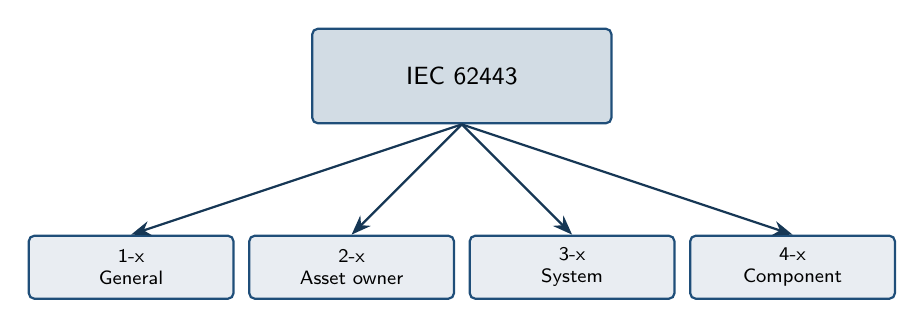
\begin{tikzpicture}[node distance=8mm]
  \node[isbox, fill=isOT!20, draw=isOT, minimum width=38mm, minimum height=12mm] (root) {IEC 62443};
  \node[isbox, fill=isOT!10, draw=isOT, below=14mm of root, xshift=-42mm, minimum width=26mm, font=\scriptsize, align=center] (g) {1-x\\General};
  \node[isbox, fill=isOT!10, draw=isOT, below=14mm of root, xshift=-14mm, minimum width=26mm, font=\scriptsize, align=center] (p) {2-x\\Asset owner};
  \node[isbox, fill=isOT!10, draw=isOT, below=14mm of root, xshift=14mm, minimum width=26mm, font=\scriptsize, align=center] (s) {3-x\\System};
  \node[isbox, fill=isOT!10, draw=isOT, below=14mm of root, xshift=42mm, minimum width=26mm, font=\scriptsize, align=center] (c) {4-x\\Component};
  \foreach \n in {g,p,s,c}{\draw[flow] (root.south) -- (\n.north);}
\end{tikzpicture}
\par\vspace{3mm}
\source{IEC 62443 series (joint with ISA/IEC) \textbar{} ISA-99 committee, ongoing.}
\note{
  IEC 62443 is the gold standard for industrial automation security and the only family written specifically for OT, but \emph{no plant on the planet is fully compliant with all 14+ parts}. The split is the load-bearing idea: 1-x concepts, 2-x for the asset owner (the utility, the factory), 3-x for the system integrator, 4-x for the component vendor (the PLC, the HMI). Use this to push back on vendor marketing: a PLC cannot be \emph{62443 compliant} on its own --- it can only be \emph{62443-4-2 certified}. Ask the class: if you are the operator of a wastewater plant, which parts are \emph{your} legal and contractual responsibility?
}
\end{frame}

\begin{frame}{IEC 62443 Security Levels}
\centering
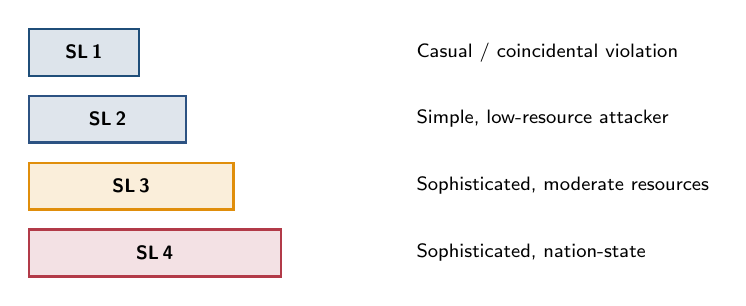
\begin{tikzpicture}[x=1cm, y=0.85cm]
  \foreach \sl/\name/\col in {
    1/{Casual / coincidental violation}/isOT,
    2/{Simple, low-resource attacker}/isPLC,
    3/{Sophisticated, moderate resources}/isAccent,
    4/{Sophisticated, nation-state}/isAttack}{
    \pgfmathsetmacro{\w}{1.4 + (\sl-1)*0.6}
    \draw[fill=\col!15, draw=\col, thick] (0, -\sl) rectangle (\w, -\sl+0.7);
    \node[font=\scriptsize\bfseries, anchor=center] at (\w/2, -\sl+0.35) {SL\,\sl};
    \node[font=\scriptsize, anchor=west] at (4.8, -\sl+0.35) {\name};
  }
\end{tikzpicture}
\par\vspace{2mm}
\begin{notebox}{Per-zone target}
Each zone gets a target SL (SL-T) chosen by \emph{consequence} and the expected \emph{threat actor}.
\end{notebox}
\note{
  The SL scale is an \emph{attacker model}, not a feature checklist --- this is the single most-misunderstood part of 62443. SL1 is accidental misuse (an engineer who fat-fingers something), SL2 is a casual attacker with low resources, SL3 is a sophisticated actor with moderate resources, SL4 is a well-funded nation-state. Pre-empt the cynicism: SL3 is \emph{not} achievable everywhere --- for most legacy brownfield plants, SL2 is the realistic ceiling because the field devices simply cannot enforce strong authentication or cryptographic integrity. The per-zone SL-T is chosen from consequence (what happens if it fails?) plus expected threat actor. Ask: is your office printer SL1 or SL2? What about the safety PLC on a hydrogen line?
}
\end{frame}

\begin{frame}{NIST Cybersecurity Framework}
\centering
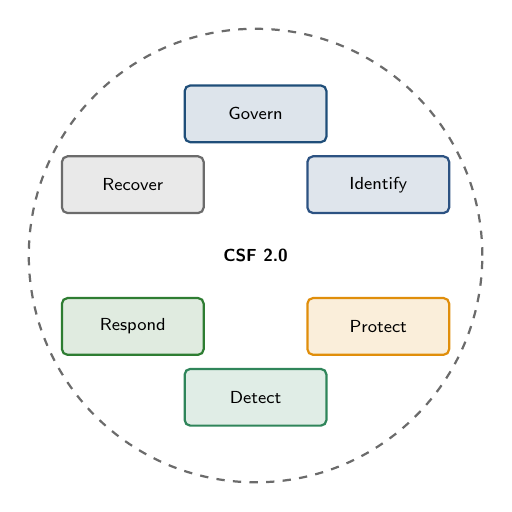
\begin{tikzpicture}[scale=0.9, transform shape]
  \def\R{2.0}
  \foreach \deg/\name/\col in {
    90/Govern/isOT,
    30/Identify/isPLC,
    330/Protect/isAccent,
    270/Detect/isHMI,
    210/Respond/isNet,
    150/Recover/isMute}{
    \node[isbox, fill=\col!15, draw=\col, font=\scriptsize, minimum width=20mm]
      at (\deg:\R) {\name};
  }
  \draw[thick, isMute, dashed] (0,0) circle (\R+1.2);
  \node[font=\scriptsize\bfseries] at (0,0) {CSF 2.0};
\end{tikzpicture}
\par\vspace{1mm}
{\footnotesize Outcome-based, sector-neutral. NIST SP 800-82 Rev.\,3 is the ICS-specific companion.}
\source{NIST, \emph{Cybersecurity Framework 2.0}, Feb 2024 \textbar{} NIST SP 800-82 Rev.\,3, Sep 2023.}
\note{
  CSF 2.0 added \emph{Govern} as a sixth function in February 2024 --- before that, governance was buried inside Identify, which let boards pretend it was an IT problem. The CSF is outcome-based and sector-neutral: it tells you \emph{what} to achieve, not \emph{how}. NIST SP 800-82 Rev.\,3 (September 2023) is the OT-specific companion that maps CSF outcomes to ICS realities --- e.g., \emph{Detect} on a serial Modbus link does not look like \emph{Detect} on an enterprise LAN. Common pairing in industry: CSF for the board slides, 62443 for the engineering work, 800-82 to translate between them.
}
\end{frame}

\section{Regulations}

\begin{frame}{Sectoral \& Regional Regulations}
\centering
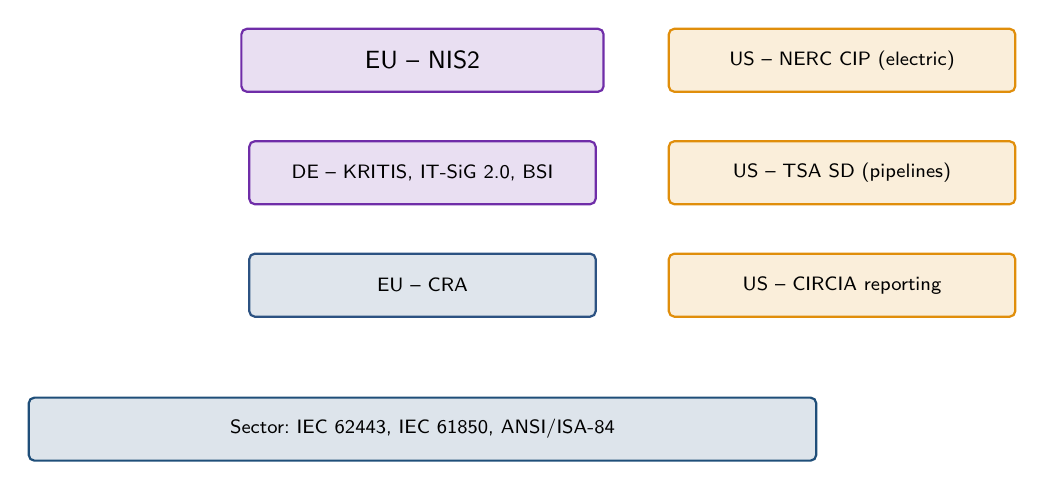
\begin{tikzpicture}[node distance=6mm]
  \node[isbox, fill=isIT!15, draw=isIT, minimum width=46mm] (eu) {EU -- NIS2};
  \node[isbox, fill=isIT!15, draw=isIT, minimum width=44mm, below=of eu, font=\scriptsize] (de) {DE -- KRITIS, IT-SiG 2.0, BSI};
  \node[isbox, fill=isPLC!15, draw=isPLC, minimum width=44mm, below=of de, font=\scriptsize] (cira) {EU -- CRA};
  \node[isbox, fill=isAccent!15, draw=isAccent, minimum width=44mm, right=8mm of eu, font=\scriptsize] (us1) {US -- NERC CIP (electric)};
  \node[isbox, fill=isAccent!15, draw=isAccent, minimum width=44mm, below=of us1, font=\scriptsize] (us2) {US -- TSA SD (pipelines)};
  \node[isbox, fill=isAccent!15, draw=isAccent, minimum width=44mm, below=of us2, font=\scriptsize] (us3) {US -- CIRCIA reporting};
  \node[isbox, fill=isOT!15, draw=isOT, minimum width=100mm, below=10mm of cira, font=\scriptsize] (sec)
    {Sector: IEC 62443, IEC 61850, ANSI/ISA-84};
\end{tikzpicture}
\source{NIS2: Directive (EU) 2022/2555 \textbar{} CRA: Regulation (EU) 2024/2847 \textbar{} KRITIS: BSI-Kritisverordnung \textbar{} NERC CIP-002--CIP-014.}
\note{
  Two dates students should memorise: NIS2 (Directive (EU) 2022/2555) transposition deadline was 17 October 2024 --- most member states missed it, but the duties apply anyway. The CRA (Regulation (EU) 2024/2847) was signed 23 October 2024 and most provisions enter force on 11 December 2027, with vulnerability-reporting duties biting earlier. KRITIS has had real teeth in Germany since 2015 via the IT-Sicherheitsgesetz and the BSI-Kritisverordnung; thresholds dropped significantly under IT-SiG 2.0. On the US side, NERC CIP (CIP-002 through CIP-014) is the only mandatory cyber regime with multi-million-dollar fines per violation per day --- the electric sector takes it seriously. Transition cue: \emph{your factory in Stuttgart making car parts --- which of these apply?} Answer: probably not KRITIS (below thresholds), maybe NIS2 (manufacturing of motor vehicles is an Annex II \emph{important entity} sector), definitely CRA the moment you ship a connected product.
}
\end{frame}

\section{Programme}

\begin{frame}{Building an OT Security Programme}
\vspace{-2mm}
\centering
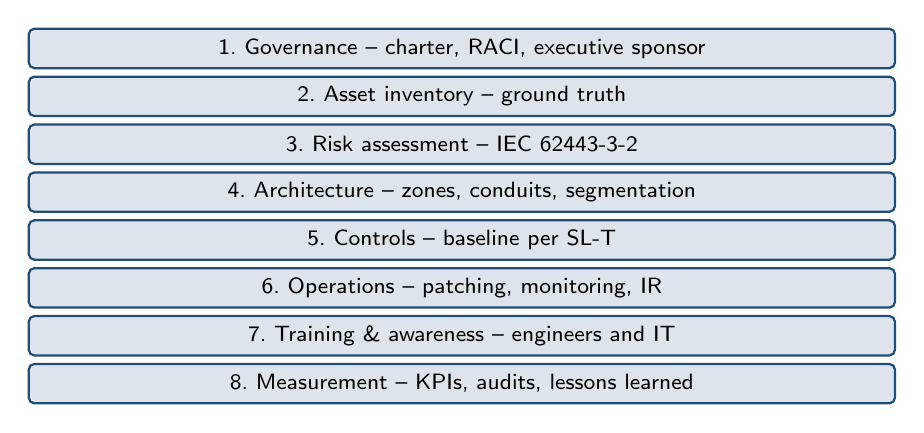
\begin{tikzpicture}[node distance=0.8mm]
  \node[isbox, fill=isOT!15, draw=isOT, minimum width=110mm, minimum height=5mm, font=\footnotesize] (a) {1. Governance -- charter, RACI, executive sponsor};
  \node[isbox, fill=isOT!15, draw=isOT, minimum width=110mm, minimum height=5mm, font=\footnotesize, below=of a] (b) {2. Asset inventory -- ground truth};
  \node[isbox, fill=isOT!15, draw=isOT, minimum width=110mm, minimum height=5mm, font=\footnotesize, below=of b] (c) {3. Risk assessment -- IEC 62443-3-2};
  \node[isbox, fill=isOT!15, draw=isOT, minimum width=110mm, minimum height=5mm, font=\footnotesize, below=of c] (d) {4. Architecture -- zones, conduits, segmentation};
  \node[isbox, fill=isOT!15, draw=isOT, minimum width=110mm, minimum height=5mm, font=\footnotesize, below=of d] (e) {5. Controls -- baseline per SL-T};
  \node[isbox, fill=isOT!15, draw=isOT, minimum width=110mm, minimum height=5mm, font=\footnotesize, below=of e] (f) {6. Operations -- patching, monitoring, IR};
  \node[isbox, fill=isOT!15, draw=isOT, minimum width=110mm, minimum height=5mm, font=\footnotesize, below=of f] (g) {7. Training \& awareness -- engineers and IT};
  \node[isbox, fill=isOT!15, draw=isOT, minimum width=110mm, minimum height=5mm, font=\footnotesize, below=of g] (h) {8. Measurement -- KPIs, audits, lessons learned};
\end{tikzpicture}
\note{
  This is the operational shape of any 62443-2-1 programme. The order matters: governance first, because without an executive sponsor the rest dies in a budget review; asset inventory second, because you cannot protect what you do not know exists --- and most operators discover 20--40\% more devices than they expected on day one. Risk assessment per 62443-3-2 produces the zones, conduits, and SL-Ts that drive every downstream decision. Pre-empt the cynicism here too: \emph{compliance is not security} --- but skipping any of these eight rows is exactly how breaches happen. Ask: in a 200-person engineering plant, who actually owns step 1?
}
\end{frame}

\begin{frame}{IEC 62443-2-1 -- Asset Owner Programme}
\centering
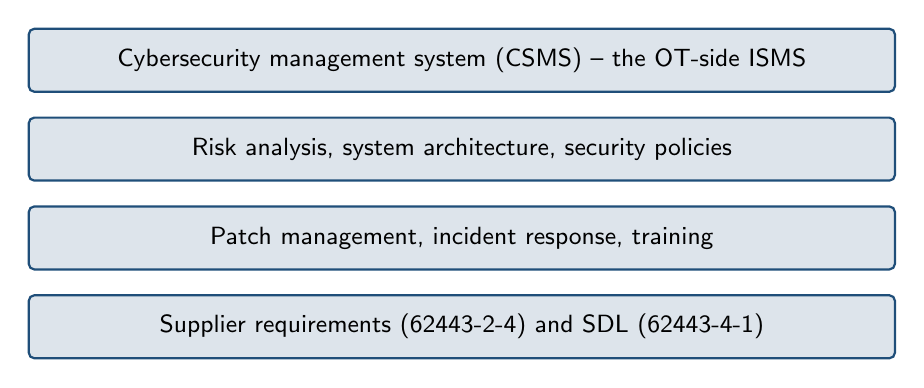
\begin{tikzpicture}[node distance=3mm]
  \node[isbox, fill=isOT!15, draw=isOT, minimum width=110mm, font=\small] (a) {Cybersecurity management system (CSMS) -- the OT-side ISMS};
  \node[isbox, fill=isOT!15, draw=isOT, minimum width=110mm, font=\small, below=of a] (b) {Risk analysis, system architecture, security policies};
  \node[isbox, fill=isOT!15, draw=isOT, minimum width=110mm, font=\small, below=of b] (c) {Patch management, incident response, training};
  \node[isbox, fill=isOT!15, draw=isOT, minimum width=110mm, font=\small, below=of c] (d) {Supplier requirements (62443-2-4) and SDL (62443-4-1)};
\end{tikzpicture}
\vspace{2mm}
\begin{notebox}{For asset owners}
2-1 is the part you implement as a utility or operator. It is the auditable backbone.
\end{notebox}
\note{
  62443-2-1 is the OT-side equivalent of ISO/IEC 27001 --- a cybersecurity management system (CSMS) with policies, processes, and evidence. If your customer asks \emph{are you 62443 compliant?} as an operator, what they really want to see is a 2-1 conformance statement plus your 3-2 risk assessment. The supplier requirements in 62443-2-4 are how you push security duties down your supply chain --- in EU contracts post-NIS2, this is increasingly contractual rather than optional. 4-1 (the secure development lifecycle) is the vendor mirror: SBOM, threat modelling, vulnerability handling. Note that 2-1 was substantially revised in 2024 to align with NIS2 and the CRA's vendor duties.
}
\end{frame}

\begin{frame}{IEC 62443-4-2 -- Component Requirements}
\centering
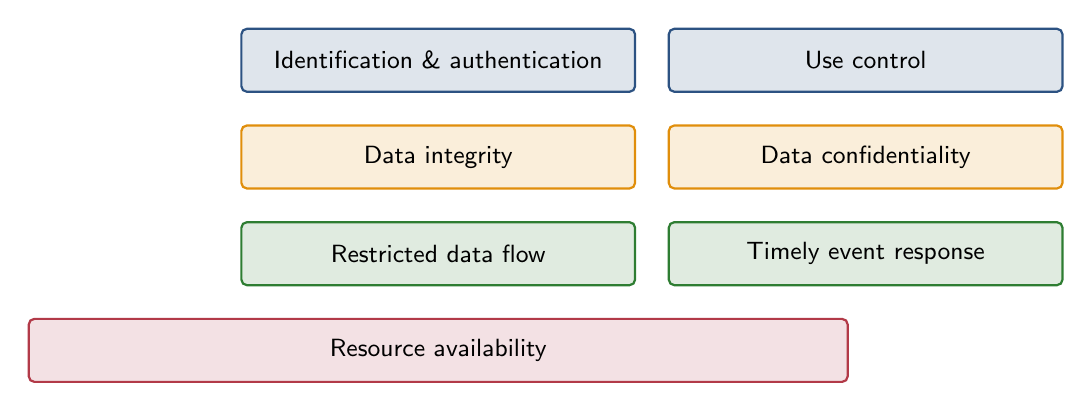
\begin{tikzpicture}[node distance=4mm]
  \node[isbox, fill=isPLC!15, draw=isPLC, minimum width=50mm, font=\small] (id) {Identification \& authentication};
  \node[isbox, fill=isPLC!15, draw=isPLC, minimum width=50mm, font=\small, right=of id] (uc) {Use control};
  \node[isbox, fill=isAccent!15, draw=isAccent, minimum width=50mm, font=\small, below=of id] (di) {Data integrity};
  \node[isbox, fill=isAccent!15, draw=isAccent, minimum width=50mm, font=\small, right=of di] (dc) {Data confidentiality};
  \node[isbox, fill=isNet!15, draw=isNet, minimum width=50mm, font=\small, below=of di] (rd) {Restricted data flow};
  \node[isbox, fill=isNet!15, draw=isNet, minimum width=50mm, font=\small, right=of rd] (te) {Timely event response};
  \node[isbox, fill=isAttack!15, draw=isAttack, minimum width=104mm, font=\small, below=of rd] (ra) {Resource availability};
\end{tikzpicture}
\par\vspace{2mm}
{\footnotesize Seven Foundational Requirements (FRs), each refined into System Requirements (SRs) per SL.}
\note{
  These seven Foundational Requirements (FRs) are the universal vocabulary of OT security --- once you internalise them, every vendor datasheet starts to make sense. Each FR breaks into Component Requirements (CRs) and System Requirements (SRs), and each requirement is repeated at SL1, SL2, SL3, SL4 with increasing rigor. Example: \emph{Identification \& authentication} at SL1 might mean shared passwords, at SL2 unique users, at SL3 multi-factor, at SL4 cryptographically bound hardware tokens. Resource availability is the odd one out --- it is the FR most directly tied to safety and the one IT security people consistently underestimate. When you certify a PLC, you certify it \emph{against a specific SL across these seven FRs} --- often SL2-capable for most FRs, SL1 for one or two stragglers.
}
\end{frame}

\begin{frame}{NIST SP 800-82 Rev.\,3}
\begin{itemize}
  \item ICS-specific companion to NIST SP 800-53.
  \item Published 2023; mapping tables to IEC 62443 included.
  \item Tiered guidance: low / moderate / high impact systems.
  \item Strong focus on \textbf{safety} and \textbf{operational continuity} -- not just confidentiality.
\end{itemize}
\vspace{2mm}
\begin{notebox}{When to reach for it}
US federal contractors, sector-CISA regulated entities, and any team that prefers outcome-based controls to a prescriptive standard.
\end{notebox}
\note{
  SP 800-82 Rev.\,3 (September 2023) is the long-awaited rewrite that finally brings ICS guidance in line with the modern threat landscape --- it has explicit chapters on cloud-connected OT, 5G, and zero-trust patterns. The mapping tables to 62443 are gold: they let a US team that lives in NIST-land talk to a European partner that lives in IEC-land without translating from scratch. The safety-first framing is the genuine differentiator from IT security guidance --- it accepts that you cannot simply reboot a turbine to apply a patch. Reach for 800-82 when you want \emph{outcomes with examples} rather than the more bureaucratic 62443 conformance language.
}
\end{frame}

\begin{frame}{EU Cyber Resilience Act (CRA)}
\centering
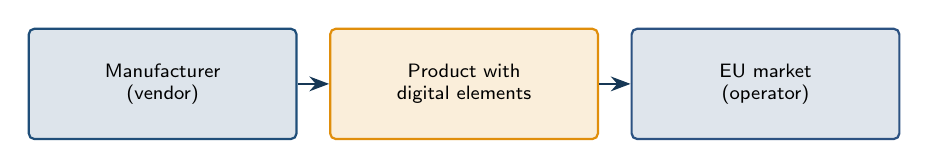
\begin{tikzpicture}[node distance=4mm]
  \node[isbox, fill=isOT!15, draw=isOT, minimum width=34mm, minimum height=14mm, align=center, font=\scriptsize] (m) {Manufacturer\\(vendor)};
  \node[isbox, fill=isAccent!15, draw=isAccent, minimum width=34mm, minimum height=14mm, align=center, font=\scriptsize, right=of m] (p) {Product with\\digital elements};
  \node[isbox, fill=isPLC!15, draw=isPLC, minimum width=34mm, minimum height=14mm, align=center, font=\scriptsize, right=of p] (u) {EU market\\(operator)};
  \draw[flow] (m) -- (p); \draw[flow] (p) -- (u);
\end{tikzpicture}
\vspace{2mm}
\begin{importantbox}{New duties}
Manufacturers must provide security updates, vulnerability handling, and an SBOM. CE marking now covers cybersecurity too.
\end{importantbox}
\source{Regulation (EU) 2024/2847 of the European Parliament and Council (Cyber Resilience Act), 23 Oct 2024.}
\note{
  The CRA is the EU's answer to \emph{ship-and-forget} vendors: any \emph{product with digital elements} placed on the EU market --- a PLC, a router, a smart sensor, even a software library --- now carries lifetime cybersecurity duties. Manufacturers must provide security updates for the expected product lifetime (default 5 years), publish an SBOM, run a coordinated vulnerability disclosure process, and report actively exploited vulnerabilities to ENISA within 24 hours. CE marking now legally covers cybersecurity, which means market surveillance authorities can pull non-compliant products from shelves. Most provisions enter force 11 December 2027; vulnerability-reporting duties bite earlier in September 2026. For OT vendors this is genuinely transformational --- the days of selling a PLC with a 15-year support tail and no patches are over.
}
\end{frame}

\begin{frame}{ENISA OT Recommendations}
\begin{itemize}
  \item Risk-based, sector-tailored controls (energy, transport, water).
  \item Strong emphasis on \emph{supply chain} obligations.
  \item Continuous monitoring (network + endpoint) for OT estates.
  \item Cross-border incident-information-sharing framework.
\end{itemize}
\begin{notebox}{For EU operators}
ENISA guidance is non-binding but shapes how national CERTs read NIS2 duties.
\end{notebox}
\note{
  ENISA does not regulate but it heavily influences --- the \emph{Good practices for the security of IACS} series (2020 onwards) is the de-facto reference national CERTs and CSIRTs cite when interpreting NIS2 \emph{appropriate measures}. The supply-chain emphasis matches CRA's manufacturer duties: an operator is now expected to demand SBOM and vulnerability-handling evidence from suppliers and to record it. Continuous monitoring as ENISA defines it is broader than IDS --- it includes asset-discovery delta tracking, configuration drift, and behavioural anomaly detection on OT protocols (Modbus, S7, DNP3). The cross-border framework matters because incidents in OT often span jurisdictions --- a water-utility breach in Bavaria can quickly become a federal and EU-level reporting event under NIS2 Article 23.
}
\end{frame}

\begin{frame}{Maturity Models in OT}
\centering
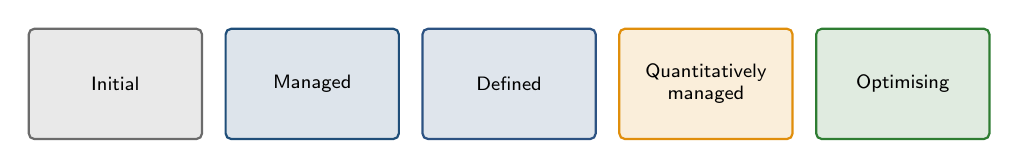
\begin{tikzpicture}[x=2.5cm]
  \foreach \i/\name/\col in {
    0/Initial/isMute,
    1/Managed/isOT,
    2/Defined/isPLC,
    3/{Quantitatively\\managed}/isAccent,
    4/Optimising/isNet}{
    \node[isbox, fill=\col!15, draw=\col, font=\scriptsize, minimum width=22mm, minimum height=14mm, align=center]
      at (\i,0) {\name};
  }
\end{tikzpicture}
\par\vspace{2mm}
{\footnotesize Common references: \textbf{C2M2} (DOE), \textbf{CMMC} (US DoD), and IEC 62443's own programme maturity.}
\note{
  Maturity models answer a different question than control frameworks: not \emph{do you do X?} but \emph{how reliably and repeatably do you do X?}. C2M2 (the US Department of Energy's Cybersecurity Capability Maturity Model) is the most-used one in critical-infrastructure self-assessments --- it is free, self-administered, and produces a defensible heatmap. CMMC is the US Department of Defense version with mandatory third-party certification for contractors. Most plants land at Managed (level 1) or Defined (level 2); reaching Quantitatively Managed requires real telemetry on security KPIs that very few OT teams have. The honest message to engineering teams: aim for level 2 with evidence rather than level 3 with hand-waving --- auditors and incident responders will both appreciate the difference.
}
\end{frame}

\begin{frame}{Audit Preparation Checklist}
\begin{itemize}
  \item Up-to-date asset inventory with firmware versions
  \item Documented zones \& conduits (preferably in a CMDB)
  \item Risk register with named owners and review dates
  \item Patch and change-management records
  \item Backup logs with restore-test evidence
  \item Incident-response playbooks plus a recent tabletop report
  \item Training attendance for operators and engineers
\end{itemize}
\begin{tipbox}{Tip}
The first audit is hardest. Treat it as a baseline scan -- gaps you find are not failures, they are your roadmap.
\end{tipbox}
\note{
  This list is what a NIS2 supervisory authority, a NERC CIP auditor, or a 62443-2-1 assessor will actually ask to see --- in roughly this order. The most common failure modes: an asset inventory that is six months stale, zones-and-conduits that exist on a PowerPoint slide but not in a CMDB, and backup logs without restore-test evidence (a backup you have never restored is a wish, not a backup). The tabletop report is often the cheapest single artefact to produce and the one that most impresses auditors --- two hours of structured discussion with operators creates more security uplift than a quarter of patching. Emphasise the tip: the first audit is a baseline, not a verdict --- the regulator's job is partly to help you produce a credible roadmap.
}
\end{frame}

\begin{frame}{Summary -- Section \sectionNumber}
\begin{takeawaybox}{What to remember from this section}
\begin{itemize}\setlength{\itemsep}{2pt}
  \item IEC 62443 provides the engineering vocabulary; NIST CSF gives the outcomes language.
  \item Security Levels (SL 1--4) tie risk to required control rigor.
  \item Regulations now demand board-level accountability and incident reporting.
  \item A programme is governance, inventory, risk, architecture, controls, ops, training, measurement.
\end{itemize}
\end{takeawaybox}
\note{
  The four take-aways are the absolute minimum a graduate of this lecture should be able to recite at a job interview. If a candidate cannot distinguish the engineering vocabulary (62443 zones, conduits, SLs) from the outcomes vocabulary (CSF Govern--Identify--Protect--Detect--Respond--Recover), they will struggle in any cross-functional OT security role. Reinforce the single most important industry truism one more time: \emph{compliance is not security}, but every breach post-mortem of the last decade reads like a list of skipped 62443 foundational requirements. Post-NIS2 and post-CRA, board-level accountability and 24-hour incident reporting are no longer optional --- treat them as design constraints from day one. Final transition: next section we move from \emph{what should we do?} into \emph{how do we actually defend a live process?}
}
\end{frame}

\referencesframe{
  \item IEC 62443 series. \emph{Industrial communication networks -- IT security for networks and systems} (joint ISA/IEC).
  \item NIST. \emph{Cybersecurity Framework 2.0}, Feb 2024.
  \item Stouffer, K. et al. \emph{NIST SP 800-82 Rev.\,3 -- Guide to OT Security}, Sep 2023.
  \item NIST SP 800-53 Rev.\,5. \emph{Security and Privacy Controls for Information Systems and Organizations}, 2020.
  \item Directive (EU) 2022/2555. \emph{NIS2 Directive}, 14 Dec 2022.
  \item Regulation (EU) 2024/2847. \emph{Cyber Resilience Act}, 23 Oct 2024.
  \item Germany BSI. \emph{BSI-Kritisverordnung (BSI-KritisV)} and \emph{IT-Sicherheitsgesetz 2.0}.
  \item ENISA. \emph{Good practices for the security of IACS}, 2020 onwards.
  \item NERC. \emph{CIP Reliability Standards}, CIP-002 through CIP-014.
  \item US TSA. \emph{Pipeline / Rail Security Directives}, 2021 onwards.
  \item US CISA. \emph{CIRCIA -- Cyber Incident Reporting for Critical Infrastructure Act}, in rule-making.
  \item DOE. \emph{Cybersecurity Capability Maturity Model (C2M2)}, current.
}

\closingframe

\end{document}
